%\documentclass[onecolumn]{IEEEtran}
%anonymous,review,
\documentclass[anonymous,review,acmsmall,10pt]{acmart}
%\usepackage[nonatbib,preprint]{neurips_2020}
%\usepackage{natbib} 
%\usepackage[dvipsnames]{xcolor}
\definecolor{LGray}{gray}{0.98}
\definecolor{dgray}{gray}{0.3}
\usepackage[utf8]{inputenc}

\usepackage{IEEEtrantools}
%\usepackage{standalone}
%\include{examplepreamble}
%\standaloneconfig{}
%\usepackage[subpreambles=true]{standalone}
\usepackage{import}
\usepackage{framed}

%\usepackage[hidelinks]{hyperref}

%\usepackage{cite}

\usepackage{caption}
%\usepackage{graphicx}
%\usepackage{float}
%\usepackage{listing}

%\usepackage{scrextend}
\usepackage{hyperref}
\renewcommand\UrlFont{\color{blue}\rmfamily}
\hypersetup{
	colorlinks=true,
	linkcolor=dgray,
	filecolor=magenta,      
	urlcolor=blue,
	citecolor=dgray,
}




%%% for code wraping
\usepackage{minted}
\usemintedstyle{colorful}
\setminted[julia]{frame=lines,rulecolor=dgray,bgcolor=LGray,fontsize=\footnotesize ,breaklines}
\usepackage{tikz}
\usetikzlibrary{shapes.geometric, arrows}
\usetikzlibrary{mindmap}

\tikzstyle{layer} = [rectangle, rounded corners, minimum width=3cm, minimum height=1cm,text centered, draw=black]
\tikzstyle{arrow} = [thick,->,>=stealth]


\usepackage{pmboxdraw}
%\usepackage{qtree}
%\usepackage{subcaption}


\usepackage{array}
\usepackage{multirow}

\title{NumNN: Conventional Neural Networks on Non-Conventional Arithmetic}

\author{Mohammad Hizzani}
\orcid{0000-0002-7734-8473}
\affiliation{%
	\department{INESC-ID}
	\department{Instituto Superior Técnico}
	\institution{University of Lisbon}
	%\streetaddress{Rua Alves Redol 9}
	%\postcode{1000-029}
	\city{Lisbon}
	\country{Portugal}
}
\email{moh.hizzani@gmail.com}


\author{Leonel Sousa}
\affiliation{%
	\department{INESC-ID}
	\department{Instituto Superior Técnico}
	\institution{University of Lisbon}
	\streetaddress{Rua Alves Redol 9}
	\postcode{1000-029}
	\city{Lisbon}
	\country{Portugal}
}
\orcid{0000-0002-8066-221X}
	%\IEEEauthorblockN
	%Mohammad~Hizzani,%\\
	%\inst{1}%\orcidID{0000-0002-7734-8473}
	%\IEEEauthorblockA
	%{
	%INESC-ID\\ 
	%Instituto Superior Técnico\\ 
	%	Universidade de Lisboa\\
	%	Email: \href{mailto:moh.hizzani@gmail.com}{\tt moh.hizzani@gmail.com}%}
	%\and
	%\IEEEauthorblockN
	%Leonel~Sousa%\\
	%\inst{1}%\orcidID{0000-0002-8066-221X}
	%\IEEEauthorblockA
	%{
	%INESC-ID\\ 
	%	Instituto Superior Técnico\\ 
	%	Universidade de Lisboa\\
	%	Email: \href{mailto:las@inesc-id.pt}{\tt las@inesc-id.pt}%}
	%Email: some@sdf.com}
%}
%
%\authorrunning{M. Hizzani and L. Sousa}
%
%\institute{Universidade de Lisboa Instituto Superior Técnico, Lisboa, Lisboa, PT
%\email{moh.hizzani@gmail.com}%
%\\
\email{las@inesc-id.pt}


\begin{document}

	\begin{abstract}
		As the development of Deep Neural Networks models increases in terms of complexity and deep architectures organized around different number of layers, whether they are fully-connected networks or convolutional, a crucial need for hardware support boosts. In addition, deep learning models use big data for training, also, with the need for tuning the hyper parameters, which requires the repetition of the whole training process multiple times. Thus, hardware-friendly number systems and arithmetic operations have been introduced alternatively to the IEEE floating-point formats and conventional arithmetic, which are cost-effective and/or more accurate. However, the hardware design, verification and assessment are complex and expensive processes. Hence, these arithmetic systems should be tested in simulation environments for the target applications, before moving forward to system design. Most deep learning frameworks and libraries target AI production, they are only supporting the IEEE floating point formats. This paper presents NumNN, a tool for facilitating the design and prototyping of deep learning systems based on different number representations, or the simulation of new hardware-oriented arithmetic operations. It provides an agile way of designing, training and evaluating any type of deep learning (neural network) model with any number system. NumNN has been used to develop deeplearning networks supported not only on 32-bit and 64-bit IEEE floating point formats but also on the Posit number representation.  Results, obtained with NumNN for benchmarks, are presented and compared with TensorFlow, showing the practical interest of the proposed software tool.
	\end{abstract}

\begin{CCSXML}
	<ccs2012>
	<concept>
	<concept_id>10010583.10010717.10010721</concept_id>
	<concept_desc>Hardware~Functional verification</concept_desc>
	<concept_significance>500</concept_significance>
	</concept>
	<concept>
	<concept_id>10010147.10010178</concept_id>
	<concept_desc>Computing methodologies~Artificial intelligence</concept_desc>
	<concept_significance>500</concept_significance>
	</concept>
	<concept>
	<concept_id>10010147.10010341.10010366.10010367</concept_id>
	<concept_desc>Computing methodologies~Simulation environments</concept_desc>
	<concept_significance>500</concept_significance>
	</concept>
	</ccs2012>
\end{CCSXML}

\ccsdesc[500]{Hardware~Functional verification}
\ccsdesc[500]{Computing methodologies~Artificial intelligence}
\ccsdesc[500]{Computing methodologies~Simulation environments}

	\maketitle

	\section{Introduction}

%\IEEEPARstart{M}{any}
Many new and old number systems have been introduced as a better alternative to IEEE-754 standards \cite{754} in the field of Deeplearning. Some were used in many different fields of Digital Signal Processing (DSP) or other specific application systems and for the sake of neural networks they have been modified to process all or some types of neural networks (i.e. Fully-connected layers, CNN and RNN).

\subsection{Examples of Number Systems Used in Deeplearning}

An example of novel number systems is the Posit number system \cite{Gustafson2017}, which is known also as UNUM III. Posit was introduced as an advanced number system that overpasses IEEE standards as a hardware-friendly system for general-purpose computational arithmetic operations. It also provides some faster versions of functions used in neural networks such as the Sigmoid function\footnote{Sigmoid function $\left(\sigma(x) = \frac{1}{1 + e^{-1}}\right)$ is rarely used as an activation function nowadays. However, $\tanh$ function is widely used and it is a scaled and shifted version of the Sigmoid function $\left(\tanh(x) = 2 \sigma(2x) -1\right)$.}.

Some suggest to use some previously known number systems that can be modified to perform much faster computation than the conventional IEEE-754. Residual Number System (RNS) \cite{Garner1959} has been being used in many DSP applications \cite{Cardarilli2007,Chaves2003,Claudio1995,DiClaudio1990,Jullien1987} and other extensive computational applications like asymmetric cryptography \cite{Hizzani2019,Asif2018a,Schinianakis2014,Antao2014}. RNS was used as a potential number system to provide energy-saving units in Convolution Neural Networks (CNN) \cite{Samimi2020}.

Another well-known number system is the Logarithmic Number System (LNS) \cite{Kingsbury1971,Alexopoulos1975,Lee1977} which also has been being used in many applications including DSP \cite{Dimitrov2001,Lewis1995}. Recently it has been developed to be used in CNN to provide higher accuracy in training using significantly smaller bit length \cite{Miyashita2016,Juang2019}.

\subsection{Why Julia?}

Julia \cite{Julia,Bezanson2017} is a high-level programming language that was designed with scientific research and data science in mind. It provides an unconventional way of defining primitive types at hardware level (with number of bits predefined) where all data types of Julia were defined, designed and implemented using only native Julia\footnote{\mintinline{julia}{Float16, Float32, Float64} represent the IEEE Floating types in Julia. \mintinline{julia}{Int128, Int16, Int32, Int64, Int8} are the conventional Signed-Integers similarly \mintinline{julia}{UInt128, UInt16, UInt32, UInt64, UInt8} are the conventional Unsigned integers.}.

Moreover, Julia provides a novel way of handling \emph{multiple dispatch} \cite{WikiMultipleDispatch} concept in programming languages \cite{JuliaMehtods}. Multiple Dispatch in a nutshell is that a function with a single name has different processes (methods) base on its argument(s). Examples of multiple dispatch are the primitive operations (addition, subtraction, multiplication and division) as follows:

\begin{listing}[H]
\begin{minted}{julia}
julia> aInt, bInt = 1, 2; #these are Integers

julia> aF, bF = 1.0, 2.0; #there are Floats

julia> aInt + bF #this will call the method +(::Integer, ::Float64) note the result is in Float64
3.0
\end{minted}
\caption{Multiple Dispatch First Example}
\end{listing}

Note how the result was promoted to be in \mintinline{julia}{Float64} because of Julia special promotion functions (\mintinline[fontsize=\footnotesize ]{julia}{promote_type(::Type{Integer},::Type{Float64}) = Float64}). This means that functions used in any package can be used without making any modification to the package, it is only required to define methods of those functions for the new type. For instance, functions such as Trigonometric functions or Hyperbolic functions as by default provided by Julia for its primitive types including the IEEE-754 types. If any of these are used in a package simply define any of them for the new number system that is to be used in this package, for further details see subsection~\ref{subsec:saa}.

\textbf{Divide and conquer} is an essential approach of development, which facilitates the focus on smaller pieces of a development process by dividing a system into layers, this way each layer is being studied and improved. Hence, this property of Julia (Multiple Dispatch) makes it much easier to separate different steps of development by developing a package and then integration with it will be separated of the source code. This means that less time is used on editing and modifying, and more time is used for designing, testing and developing. In the upcoming sections it will be presented what methods of functions of NumNN.jl with which any new number system should be defined beforehand.

Furthermore, Julia provides a native support for parallel operations namely co-routines, multi-threads and multi-core. Mostly no new code is needed for parallel operations, and when needed, the same code with some macros do the job. In the same way, for-loops in Julia are extremely fast as fast as for-loops of C-like languages. 

	
	\section{Structure and Organization}

The NumNN.jl  package\footnote{\url{https://github.com/MohHizzani/NumNN.jl}} (library) was built on the concept of Rapid Prototyping to enable fast experimentation. \emph{Begin able to go from idea to result with the least possible delay is key to good research} \cite{Keras}. There are so many deeplearning frameworks out on the internet \cite{Abadi2016,Collet2015,Jia2014,Paszke2017,PyTorch2019}, some are widely spread and efficient in production and research as long as you are using the IEEE-754 standards. However, most of these libraries run on Python which has not the native support of newly added primitive types nor the efficiency of Julia in multiple dispatch (i.e. any new defined number systems needs an internal modification to the library itself to be capable of handling it). Even packages of Julia like Flux.jl \cite{Flux.jl-2018,Innes2018} or Knet \cite{Yuret2016k} neither of them fully support newly added types, and do not provide the flexibility of different types for different parameters or to deliver output with certain desired data types. Thus, NumNN.jl provides a fully support for a total in one type computation, the ability to choose the type of each group of parameters and the capabilities of delivering output of a chosen type.

\subsection{Fast Implementation and Deployment}

NumNN.jl provides the fastest possible way to implement a neural network model, train and use it for prediction and testing. Installing the package and using it can be done from a Julia REPL as follows:

\begin{listing}[H]
	\begin{minted}{julia}
	julia> ] add NumNN
	julia> using NumNN
	\end{minted}
	\caption{Adding NumNN.jl and import it}\label{addimport}
\end{listing}

Defining layers sequence can be easily done either like this:

\begin{listing}[H]
	\begin{minted}{julia}
	X_Input, X_Ouput = chain(X_train,[Flatten(),FCLayer(120,:relu),FCLayer(10,:softmax)])
	\end{minted}
	\caption{Chained Layers with no side branch(es)}\label{chain}
\end{listing}


where \mintinline[fontsize=\footnotesize]{julia}{X_train} is the train array or the size of train array. Or in case there are some side branches it can be easily done as the example of Inception Net \cite{Szegedy2016} (Listing~\ref{chain}). 

%A group of examples can be found in Appendices.

\subsection{Structure and Architecture}\label{subsec:saa}

The structure of NumNN.jl is simple enough to comprehend in few minutes and to start to amend in case any new element is needed to be added. \figurename~\ref{fig:layerstruct} shows the Layers hierarchy in NumNN.jl, this structure was built to facilitate the use and the future development of NumNN.jl.

The convention of data shape to be used is (data dimension(s), channels, batch size). For instance, when using MNIST \cite{LeCun1998,LeCun1998a} data set the shape of training data will be (28,28,1,60000), where the first two dimensions are the images' dimensions the third one is number of channels and the last integer expresses the batch size.

\begin{figure}[!ht]
	\centering
	%\begin{subfigure}{0.95\textwidth}
		%\begin{enumerate}
%\qtreecenterfalse
%\item \Tree [.Layer  FCLayer Activation BatchNorm Flatten Input ]

%\item \Tree [.Layer [.MILayer AddLayer ConcatLayer ]]


%\item \Tree [.Layer [.PaddableLayer
%[.ConvLayer Conv1D Conv2D Conv3D ]
%[.PoolLayer
%[.AveragePoolLayer AveragePool1D AveragePool2D AveragePool3d ]
%[.MaxPoolLayer MaxPool1D MaxPool2d MaxPool3d ]]]]
%\end{enumerate}
%\documentclass{article}
%\usepackage{tikz}
%\usetikzlibrary{mindmap}
%\begin{document}


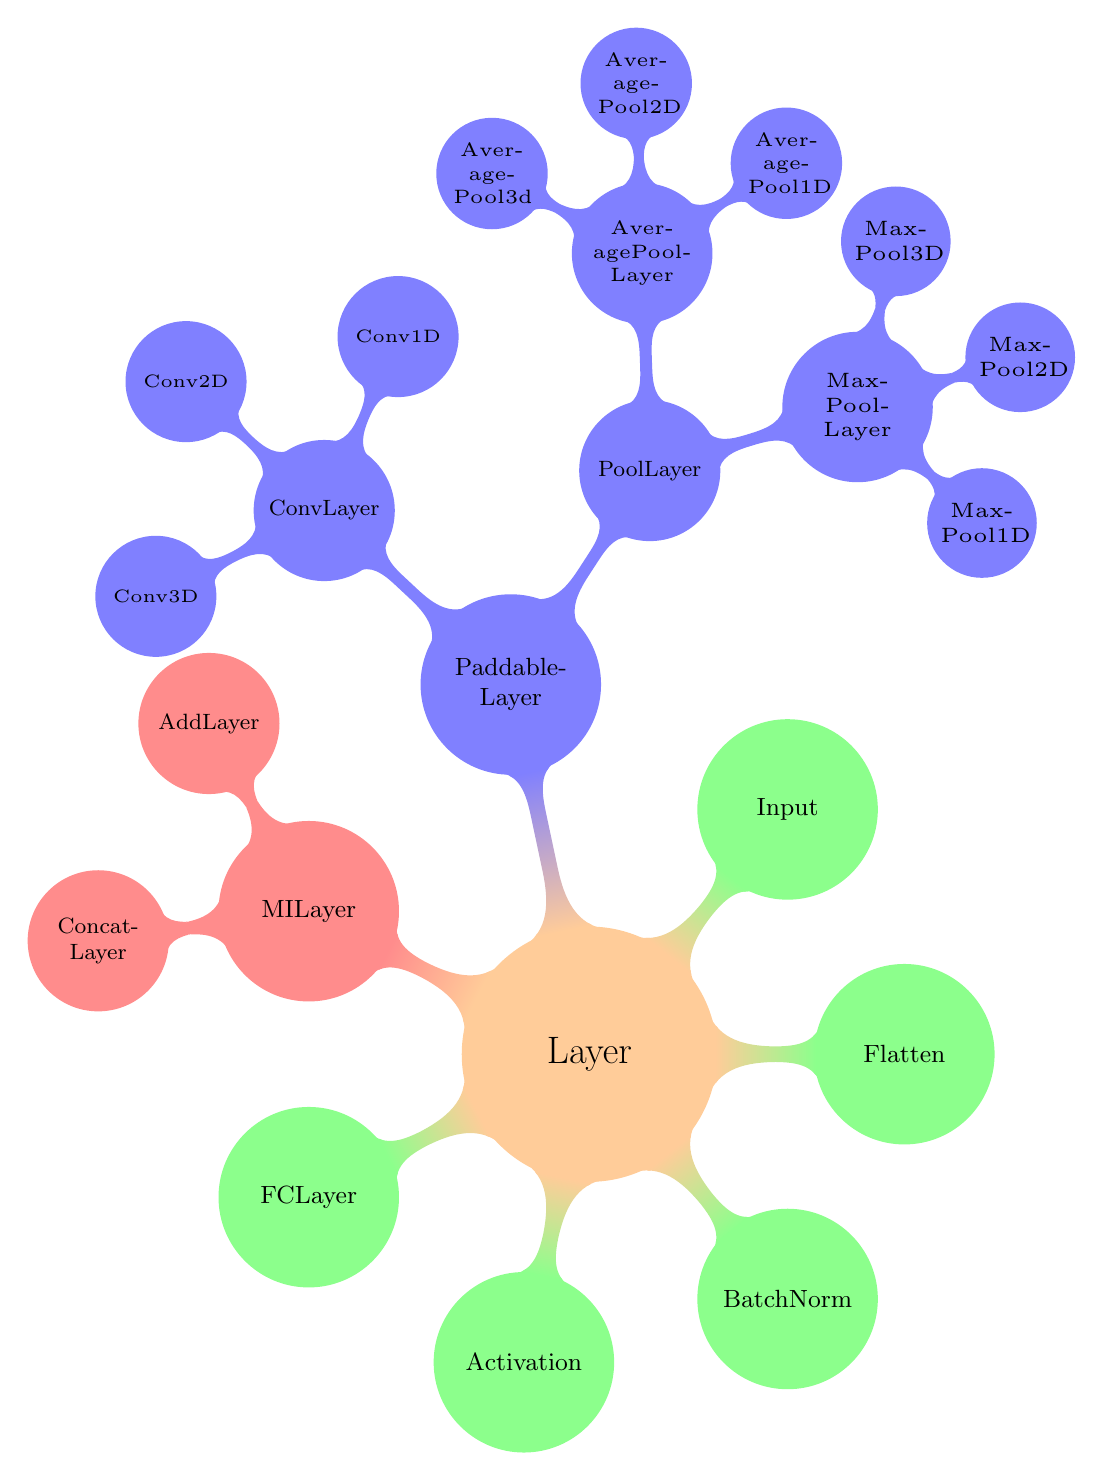
\begin{tikzpicture}[mindmap,
every node/.style={concept,
	execute at begin node=\hskip0pt}, concept color=orange!40,% concept fontsize=10pt,
grow cyclic, %text width=3cm, align=flush center,
level 1/.append style={level distance=4cm,sibling angle=51
},
level 2/.append style={level distance=2.7cm,sibling angle=70
},
level 3/.append style={level distance=2.3cm, sibling angle=70
},
level 4/.append style={level distance=1.8cm,sibling angle=60
}
%scale=0.9, transform canvas={scale=0.9}
]
\node[scale=0.8]{\LARGE Layer}
child [concept color=green!45] { node {FCLayer}}
child [concept color=green!45] { node {Activation}}
child [concept color=green!45] { node {BatchNorm}}
child [concept color=green!45] { node {Flatten}}
child [concept color=green!45] { node {Input}}
child [concept color=blue!50, scale=1.2] { node {PaddableLayer}
																	child [sibling angle=90] { node {PoolLayer}
																	child [sibling angle=80] { node [scale=1.5] {MaxPoolLayer}
																		child { node [scale=1.5] {MaxPool1D}}
																		child { node [scale=1.5] {MaxPool2D}}
																		child { node [scale=1.5] {MaxPool3D}}
																	}
																	child { node [scale=1.4] {AveragePoolLayer}
																		child { node [scale=1.4] {AveragePool1D}}
																		child { node [scale=1.4] {AveragePool2D}}
																		child { node [scale=1.4] {AveragePool3d}}
																	}
																}
																child { node {ConvLayer}
																	child [level distance=2cm] { node [scale=1.3] {Conv1D}}
																	child [level distance=2cm] { node [scale=1.3] {Conv2D}}
																	child [level distance=2cm] { node [scale=1.3] {Conv3D}}
															}}
child [concept color=red!45] { node {MILayer}
	child { node {AddLayer}}
	child { node {ConcatLayer}}
			};
\end{tikzpicture}

%\end{document}
	%\end{subfigure}
	\caption{Layer Architecture in NumNN.jl, the useable layers are the leaves the other nodes are \mintinline[fontsize=\footnotesize]{julia}{abstract type}s.}\label{fig:layerstruct}
\end{figure}

An essential data type (\mintinline[fontsize=\footnotesize]{julia}{Model}) holds the main pointers to layers structure and parameters to use. Instantiating a (\mintinline[fontsize=\footnotesize]{julia}{Model}) will also invoke the initialization of the layers scaling and bias parameters and can be done as presented in Listing~\ref{modelinit}.

\begin{listing}[H]
	\begin{minted}{julia}
	model = Model(X_train, Y_train, X_Input, X_Output, 0.001; optimizer=:adam, loss=:categoricalCrossentropy)
	\end{minted}
	\caption{Model initialization, \mintinline{julia}{X_train, Y_train} are training data and labels, while \mintinline{Julia}{X_Input, X_Ouput} are the input and output layers. The value of \mintinline{julia}{0.001} represent the learning rate of this model, where the key-word \mintinline{julia}{optimizer} define the optimizer to use during training, and \mintinline{julia}{loss} defines the loss function.}\label{modelinit}
\end{listing}

\begin{listing}[!h]
	\begin{minted}{julia}
	X_Input = Input(X_train)
	Xc = [
	Conv2D(3, (3,3), padding=:same)(X_Input),
	Conv2D(4, (5,5), padding=:same)(X_Input),
	Conv2D(10, (1,1), padding=:same)(X_Input),
	MaxPool2D((2,2); padding=:same)(X_Input),
	AveragePool2D((3,3); padding=:same)(X_Input),
	]
	X = ConcatLayer()(Xc)
	X = BatchNorm(dim=3)(X) #to normalize across the channels
	X = Activation(:relu)(X)
	X = MaxPool2D((2,2))(X);
	Xc = [
	Conv2D(6, (3,3), padding=:same)(X),
	Conv2D(8, (5,5), padding=:same)(X),
	Conv2D(10, (1,1), padding=:same)(X),
	MaxPool2D((2,2); padding=:same)(X),
	AveragePool2D((3,3); padding=:same)(X),
	]
	X = ConcatLayer()(Xc)
	X = BatchNorm(dim=3)(X) #to normalize across the channels
	X = Activation(:relu)(X)
	X = AveragePool2D((3,3))(X);
	X = Flatten()(X)
	X_Output = FCLayer(10, :softmax)(X);
	\end{minted}
	\caption{InceptionNet Example where this layer architecture has many side branches.}\label{chain}
\end{listing}

Activation functions are defined under the \mintinline[fontsize=\footnotesize]{julia}{abstract type actFun}. NumNN.jl only provided few activation functions (sigmoid ($\sigma$), \mintinline{julia}{tanh}, \mintinline[fontsize=\footnotesize]{julia}{softmax} and \mintinline[fontsize=\footnotesize]{julia}{noAct}). Using any other activation function can be defined as a subtype of \mintinline[fontsize=\footnotesize]{julia}{actFun} and then as a normal function with another function for its derivative. For instance, if you want to add $\sin$ as an activation function all what you need is expressed in Listing~\ref{newact}.

\begin{listing}[!ht]
	\begin{minted}{julia}
	abstract type sin <: actFun end
	
	sin(x) = base.sin.(x) #note the use of base. to tell julia that we need the default sin at this step not the type defined because it was overwritten
	dsin(x) = base.cos.(x)
	\end{minted}
	\caption{Example of defining a new activation function to NumNN.jl}\label{newact}
\end{listing}

NumNN.jl has loss functions under the \mintinline{julia}{abstract type lossFun}. The two main loss functions defined are the \mintinline{julia}{binaryCrossentropy} and \mintinline{julia}{categoricalCrossentropy}. Also, other loss functions can be easily defined, more functions will be available in the upcoming versions of NumNN.jl.

%\subsection{Sequence of Processes}
%The easiest way of explaining NumNN.jl is by showing a complete example. 

\subsection{Some Benchmarks and Testing}
The most convenient way to demonstrate the effectiveness of NumNN.jl is by getting hands dirty and showing some examples accompanied with comparison beside another library. Keras on the top of TensorFlow was one of the main influencers upon the syntax of NumNN.jl. Thus, some benchmarks were run on both NumNN and TensorFlow. Nonetheless, other benchmarks could not be run on TensorFlow due to lack support for new data types, therefore, they were run only on NumNN.jl.

The data used for train/test was Fashion MNIST \cite{Xiao2017}. Intel(R) Xeon(R) Gold 6140 CPU @ 2.30GHz was used for all tests, and no GPU were used (NumNN does not support GPU and other back-end so far). Table~\ref{tab:bench} shows the results of all test\footnote{All benchmarks are available at \url{https://github.com/MohHizzani/NumNN.jl/tree/master/examples}}, and where bank is present that means test was not perform under this framework because the data type is not supported\footnote{\label{batchnorm}Benchmark 2 \& 3 has Batch Normalization layer where Float64 is not supported for this layer in TensorFlow}.

\begin{table}[!ht]
	\centering
	\renewcommand{\arraystretch}{1.1}
	\caption{Various benchmarks for NumNN.jl and TensorFlow}\label{tab:bench}
	\begin{tabular}{|c | c | c || c | c |}
		\hline
		Benchmark & DType & Measurements & NumNN.jl & Tensorflow\\\hline\hline
		%%%%%%%%%% Benchmark 1
		\multirow{14}{*}{Benchmark 1} & \multirow{5}{*}{Float32} & Train Accuracy & 0.8902 & 0.9162\\
		& & Test Accuracy & 0.8650 & 0.8851\\
		& & Train Cost & 0.3000 & 0.2270\\
		& & Test Cost & 0.3728 & 0.3444\\
		& & Training Time / Sample & $84\mu$s  & $177\mu$s\\\cline{2-5}
		& \multirow{5}{*}{Float64} & Train Accuracy & 0.8812 & 0.9191 \\
		& & Test Accuracy & 0.8703 & 0.8848 \\
		& & Train Cost & 0.3314 & 0.2163 \\
		& & Test Cost & 0.3845 & 0.3311 \\
		& & Training Time / Sample & $93\mu$s & $100\mu$s\\\cline{2-5}
		& \multirow{4}{*}{Posit\{16,1\}} & Train Accuracy & 0.8716 & \rule{5em}{1pt} \\
		& & Test Accuracy & 0.8510 & \rule{5em}{1pt} \\
		& & Train Cost & 0.3520 & \rule{5em}{1pt} \\
		& & Test Cost & 0.4088 & \rule{5em}{1pt} \\\hline
		%%%%%%%%%% Benchmark 2
		\multirow{14}{*}{Benchmark 2\footref{batchnorm}} & \multirow{5}{*}{Float32} & Train Accuracy & 0.8980 & 0.9160\\
		& & Test Accuracy & 0.8786 & 0.8929\\
		& & Train Cost & 0.2760 & 0.0.2346\\
		& & Test Cost & 0.3386 & 0.2955\\
		& & Training Time / Sample & $1.31m$s & $8m$s \\\cline{2-5}
		& \multirow{5}{*}{Float64} & Train Accuracy & 0.9020 & \rule{5em}{1pt} \\
		& & Test Accuracy & 0.8857 & \rule{5em}{1pt} \\
		& & Train Cost & 0.2750 & \rule{5em}{1pt} \\
		& & Test Cost & 0.3420 & \rule{5em}{1pt} \\
		& & Training Time / Sample & $1.34m$s & \rule{5em}{1pt} \\\cline{2-5}
		& \multirow{4}{*}{Posit\{16,1\}} & Train Accuracy & 0.9114 & \rule{5em}{1pt} \\
		& & Test Accuracy & 0.8949 & \rule{5em}{1pt} \\
		& & Train Cost & 0.2453 & \rule{5em}{1pt} \\
		& & Test Cost & 0.3045 & \rule{5em}{1pt} \\\hline
		%%%%%%%%%% Benchmark 3
		\multirow{14}{*}{Benchmark 3\footref{batchnorm}} & \multirow{5}{*}{Float32} & Train Accuracy & 0.9136 & 0.9072\\
		& & Test Accuracy & 0.8953 & 0.8899\\
		& & Train Cost & 0.2362 & 0.2527\\
		& & Test Cost & 0.2962 & 0.3050\\
		& & Training Time / Sample & $3.09m$s & $14m$s\\\cline{2-5}
		& \multirow{5}{*}{Float64} & Train Accuracy & 0.9103 & \rule{5em}{1pt} \\
		& & Test Accuracy & 0.8926 & \rule{5em}{1pt} \\
		& & Train Cost & 0.2480 & \rule{5em}{1pt} \\
		& & Test Cost & 0.3067 & \rule{5em}{1pt} \\
		& & Training Time / Sample & $3.3m$s & \rule{5em}{1pt} \\\cline{2-5}
		& \multirow{4}{*}{Posit\{16,1\}} & Train Accuracy & 0.9127 & \rule{5em}{1pt} \\
		& & Test Accuracy & 0.8954 & \rule{5em}{1pt} \\
		& & Train Cost & 0.2412 & \rule{5em}{1pt} \\
		& & Test Cost & 0.2999 & \rule{5em}{1pt} \\\hline		
	\end{tabular}
\end{table}



	
	\section{Future Work}

The goal of NumNN.jl is the simplicity and generality of implementing neural networks models with the ability of adoption various number systems to be tested before the hardware design process. Moreover, NumNN.jl in the future will be able to use different back-end devices and processing units to speed up the train and inference of neural networks. 

So far, the package depends on predefined derivatives and gradients of the activation functions (each activation function has a derivative provided under the same name with the letter \mintinline{julia}{"d"} added to the front of its name like \mintinline{julia}{relu} and \mintinline{julia}{drelu}), in the upcoming versions will be able to do automated derivation and gradient techniques.

More activation functions will be added and many new loss functions to serve the easiness and generality of this package. For  the status quo NumNN.jl only accepts one input layer and one output layer, and multiple input and output layers will be of highest priority to support in the upcoming versions.
%	\includestandalone[subpreambles=true]{00-FCLayer-FashionMNIST/00-FCLayer-FashionMNIST}
	%\appendices

\section{First Example of Using NumNN.jl}\label{fenum}
%\import{00-FCLayer-FashionMNIST/}{00_FCLayer_FashionMNIST}
%\standaloneconfig{subpreambles=true}
%\includestandalone[subpreambles=true]{00-FCLayer-FashionMNIST/00-FCLayer-FashionMNIST}
%\import{00-FCLayer-FashionMNIST/}{00-FCLayer-FashionMNIST}
%\input{00-FCLayer-FashionMNIST/00-FCLayer-FashionMNIST}
	
	\bibliographystyle{ACM-Reference-Format}
	%\bibliographystyle{plain}
	\bibliography{main}
	%\printbibliography
\end{document}
